\RequirePackage[l2tabu,orthodox]{nag}
\documentclass[10pt,twocolumn,a4paper,os=win]{article}

\usepackage[utf8]{inputenc}
\usepackage[T1]{fontenc}
\usepackage[english]{babel}
\usepackage{lmodern}
\usepackage{microtype}
\usepackage{parskip}
\usepackage{amsmath}
\usepackage{csquotes}
\usepackage{graphicx}

\usepackage[
	backend=biber
]{biblatex}
\addbibresource{gui.bib}

\usepackage{menukeys}

\usepackage[hidelinks]{hyperref}

\author{Markus Himmel}
\title{Windows GUI}

\newcommand{\bs}[1]{\textbf{\sffamily #1}}
\newcommand{\winver}[1]{$^{\text{\hyperref[tbl:abbrev]{\bs{#1}}}}$}

\begin{document}
	\maketitle

	\begin{abstract}
		The Graphical User Interface is one of the most important components
		of a consumer-oriented operating system such as Microsoft Windows. This
		report examines the components of the Windows operating system that
		contribute to the graphical user interface, both from an application
		programmer's and a system architect's point of view.
	\end{abstract}

	\section{Introduction}

		Rigorously defining requirements for an efficient graphical user
		interface is outside the scope of this report. Instead, we will focus
		on one particular aspect: Responsiveness. Users perceive the response
		of a computer as \enquote{instantaneous} if the response time is less
		than 100 milliseconds \cite{miller1968response}. Ensuring that as
		little of that time as possible is used for drawing the application on
		the screen is key to the usability of a graphical user interface.

		\subsection{How to read this document}
			The Windows operating system has seen many revisions over its
			decades-long lifespan, and many of the features described in this
			report differ significantly from version to version. At the same
			time, documentation of the architecture of the Windows GUI is
			scarce at best.  For this reason, it is not possible to present an
			entirely consistent exposition of the Windows GUI architecture of
			some fixed Windows version.  Instead, different sections of this
			report may be based on different versions of Windows. In order to
			aid the reader in keeping track of which version of Windows is
			being examined at any given point in time, sections and sometimes
			single paragraphs and sentences will be marked with the Windows
			versions they describe. Here is an example:

			GDI is not hardware-accelerated.\winver{V}

			Table~\ref{tbl:abbrev} lists all abbreviations used in this document
			and the Windows versions they refer to.

			\begin{table}[h]
				\centering
				\begin{tabular}{r|l}
					Abbreviation & Windows Version \\
					\hline
					\bs{3} & Windows NT 3.51 \\
					\bs{4} & Windows NT 4.0 \\
					\bs{XP} & Windows XP \\
					\bs{V} & Windows Vista (\enquote{Longhorn}) \\
					\bs{7} & Windows 7 \\
					\\
					\bs{WRK} & Windows research kernel \\
					\bs{R} & ReactOS source code
				\end{tabular}
				\caption{Abbreviations for Windows versions used in
					this document}
				\label{tbl:abbrev}
			\end{table}

			In some cases, no documentation of a particular implementation detail
			may exist for any Windows version. In this situation, the author of
			this report used the source code of the ReactOS project in order to
			at least present \emph{a} implementation, without intending to imply
			that this implementation is similar to that of any real Windows
			version.

	\section{Win32 GUI applications}
		\subsection{Window objects}

		\subsection{Window messages and procedures}

	\section{NT Kernel support for GUI applications}
		

	\section{Win32 drawing APIs}
		\subsection{Graphics Device Interface}

		\subsection{DirectX}

		\subsection{Avalon}

		\subsection{OpenGL}

		% TODO: Vulkan, Metal, ...

	\section{Window Management}
		\subsection{Window managers and compositing}
			The window manager is the component of a window-based graphical user
			interface that is responsible for managing the position of each active
			window on the desktop and making sure the desktop as the sum of its
			parts is assembled correctly. There are two general approaches to this
			task: \emph{compositing} and \emph{non-compositing} window management.

			A non-compositing window manager draws non-window elements of the
			desktop (such as the taskbar or equivalent) and maintains the
			position and relative order of all currently visible Windows. It
			then instructs applications to draw the currently visible portion
			of their windows directly onto the screen buffer. In particular,
			this means that all applications draw to the same memory buffer and
			when a window is moved on top of another window, that window's data
			will be overwritten.

			Non-compositing window managers are efficient and relatively
			straightforward to implement. However, there are several drawbacks
			to this approach.  One such drawback is that it inherently comes
			with several visual artifacts. Because window contents are drawn
			directly on the screen without any form of dubble buffering, screen
			tearing will be visible during high-motion events such as scrolling
			text. Additionally, in a situation where a window is moved on top
			of an unresponsive window and subsequently moved away, requests to
			redraw the region of the bottom window which is now visible again
			will be sent, but not handled because the application is not
			responsive. The result is the well-known \enquote{trail} effect
			observed in old versions of Microsoft Windows. Refer to
			figure~\ref{fig:trail} for an example of the problem.
			\begin{figure}[h]
				\centering
				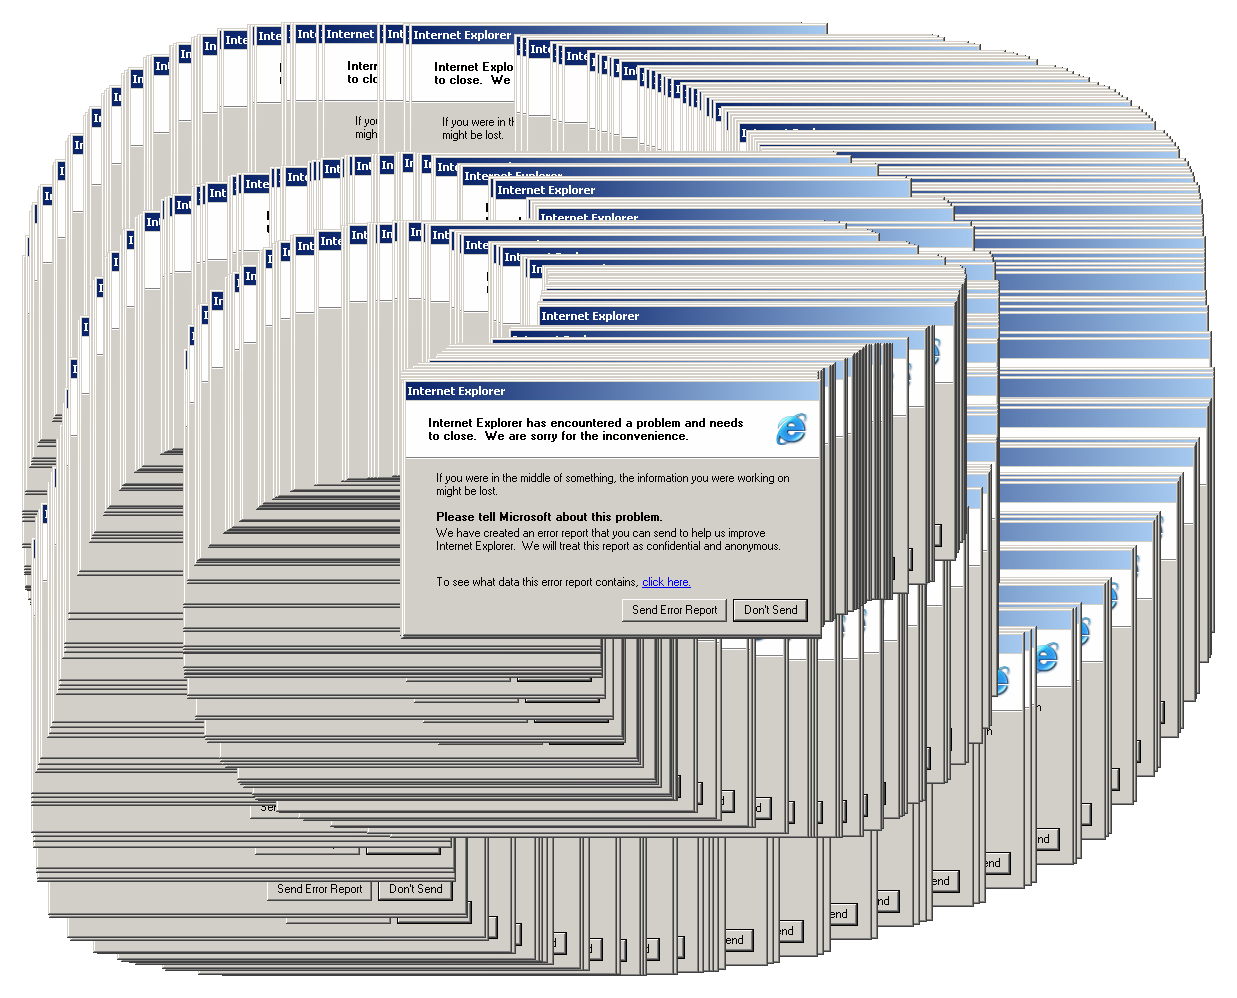
\includegraphics[width=0.8\columnwidth]{trail}
				\caption{The classic \enquote{trail} effect}
				\label{fig:trail}
			\end{figure}

			Another shortcoming of non-compositing window managers is their
			inability to provide visual effects. As a consequence of the fact
			that (at most) one application determines the color of each individual
			pixel on the screen, effects such as partially transparent windows
			cannot be realized with non-compositing window managers. Additionally,
			because a window may only be at most at one position of the screen,
			and that position has to be the Window's \enquote{actual} position,
			no thumbnails or overviews of windows can be shown.

			Compositing is an attempt at a solution to the aforementioned
			problems.  If a compositing window manager is in use, applications
			do not draw directly to the screen. Instead, each applications has
			its own off-screen buffer. The
			window manager then assembles the final
			desktop from the content of these buffers. It is immediately clear how this approach addresses the
			problems of non-compositing window-managers described above: It is
			easy to perform double buffering and even when a window is not
			responding, the window manager knows its last good state and can
			use it to prevent trails. Furthermore, visual effects are trivial
			to achieve when compositing is used. \cite{dwmoverview}

		\subsection{The Desktop Window Manager\winver{V}}
			The \emph{Desktop Window Manager} (DWM) is the compositing window
			manager used by Windows and was introduced in Longhorn
			\cite{dwmoverview}.  It is implemented as a full-screen Direct3D
			user-space application. In particular, DWM rendering is
			hardware-accelerated. When DWM is active, applications render into
			off-screen DirectX buffers which are mapped onto flat surfaces in
			3D space and rendered by the graphics hardware. This design enables
			three-dimensionally transforming the windows, which is used for the
			\enquote{Flip3D} feature of Windows Vista invoked by the keyboard
			shortcut \keys{Win+\tab} and its more modest counterparts in more
			recent versions of Microsoft Windows. Visual effects such as
			transparency are implemented using DirectX pixel shaders. In addition,
			double buffering using the a buffer flipping mechanism is implemented.
			\cite{dwmdirectx}
		\subsection{The Windows Display Driver Model\winver{V}}

		\subsection{The non-compositing window manager\winver{XP}}

	\printbibliography
\end{document}
